\section{Measuring the quirk mass and the confinement scale (P2)}\label{sec:mlam}

If a quirk signal were seen, the next questions would be its mass $\mQ$ and the string scale $\Lam$. The hit pattern
depends on them through a few combinations: $\lzero=\mQ/\Lam^2$ sets the oscillation length (Eq.~\eqref{eq:lmax}),
$\epsB\propto B/\Lam^2$ the B-field thickness (Eq.~\eqref{eq:law}), and the velocities, which depend on $\mQ$ through the
production kinematics, set the number of oscillations, the hit delays and the ionisation. This section first gives the
truth-level handles from Stage~3, which define what a detector-level measurement should be compared with, and then the
detector-level handles.

\subsection{Truth-level handles}\label{sec:mlam:truth}
The truth-level handles show what information the hit pattern carries before resolution, pile-up and reconstruction
remove part of it; each detector-level handle of Sections~\ref{sec:mlam:det} and~\ref{sec:mlam:mass} is compared with
its truth-level counterpart.
Figure~\ref{fig:edges} shows the main truth-level handles (template half of the Stage-3 sample, $|\eta_{\rm pair}|<2.5$,
smeared vertex, field and nominal material; \rep{sim/stage3/results/P2.json}).
\begin{itemize}
\item \textbf{A continuous $\Lam$ handle.} The median separation of the two quirks in the IT, $\sepIT$, scales as
  $\Lam^{-2}$ from 1 to $30\keV$ at every (species, mass) point (log-log slopes $-1.985$ to $-2.022$, each $\pm0.02$--0.04): it
  measures $\lzero=\mQ/\Lam^2$, with $\sepIT/\lmax\approx0.5$--0.6 above $1\keV$. For $E$ at $1000\GeV$ it falls from
  $38.5\mm$ at $1\keV$ to $9.3\mm$ at $2\keV$, $0.37\mm$ at $10\keV$ and $95\um$ at $20\keV$.
\item \textbf{Breaking the $(\mQ,\Lam)$ degeneracy} (truth level, \EST{}). Below $\Lcross(\mQ)$ ($1.2$--$1.9\keV$)
  the thickness is dominated by the B-field part, which depends on $\Lam$ only and is flat in $\mQ$
  (Section~\ref{sec:p1}), while $\sepIT$ measures $\mQ/\Lam^2$; at truth level the two together would separate $\mQ$
  and $\Lam$ without using the recoil. Above $\Lcross$ the thickness is set by multiple scattering and depends on
  $\mQ$. The number of tracker hits, the maximum hit delay and the fraction of pairs that do
  not turn around inside the tracker are flat in $\Lam$ and carry $\mQ$ through the velocities.
\item \textbf{Edges.} The efficiency of a coplanarity search is bounded in $\Lam$ by scales of the string
  (Fig.~\ref{fig:edges}): (i) $\Nosc=1$ at $0.28$--$0.33\keV$, independent of $\mQ$; (ii) the median $\lmax$ equals the IT
  radius at $0.43\to0.78\keV$ ($E$, $200\to1500\GeV$) and $0.59\to0.94\keV$ ($\Etil$); (iii) the median truth thickness
  (field and material) reaches $100\um$ at $0.47$--$0.55\keV$, flat in $\mQ$, the only edge tied to $\epsB$; (iv) at high
  $\Lam$ the two quirks merge into one hit: half of the pairs have an IT separation below $100\um$ at $12.8\to20.4\keV$
  ($E$) and $17.7\to25\keV$ ($\Etil$). The median $\lmax=100\um$ threshold ($16\to30\keV$ for $E$) is the same quantity
  as (ii) at another threshold: since $\lmax\propto\Lam^{-2}$, the two thresholds differ by the fixed ratio
  $\sqrt{\RIT/100\um}=\sqrt{1465}=38.2$. The $\mQ$ dependence of the $\lmax$ edges is
  $d\ln\Lam/d\ln\mQ=0.249\pm0.019$, half of the naive $\sqrt{\mQ}$ scaling, because heavier pairs are produced with
  smaller $\gst$.
\item \textbf{Edge systematics.} Varying $\lmax$ by $\pm5\%$, QED radiation, scales, PDFs, the merging scale and the
  material by $\times0.5$/$\times2$ moves the edges by a median of 2.3--5.2\% per edge type and at most 8.1\%; these are
  noise-limited upper bounds (\EST{}).
\end{itemize}

\begin{figure}[htbp]
\centering
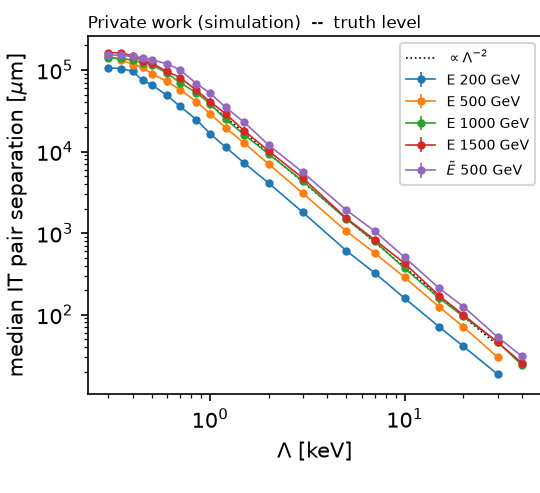
\includegraphics[height=0.37\linewidth]{figures/S3_p2_sepIT.png}\hspace{0.02\linewidth}
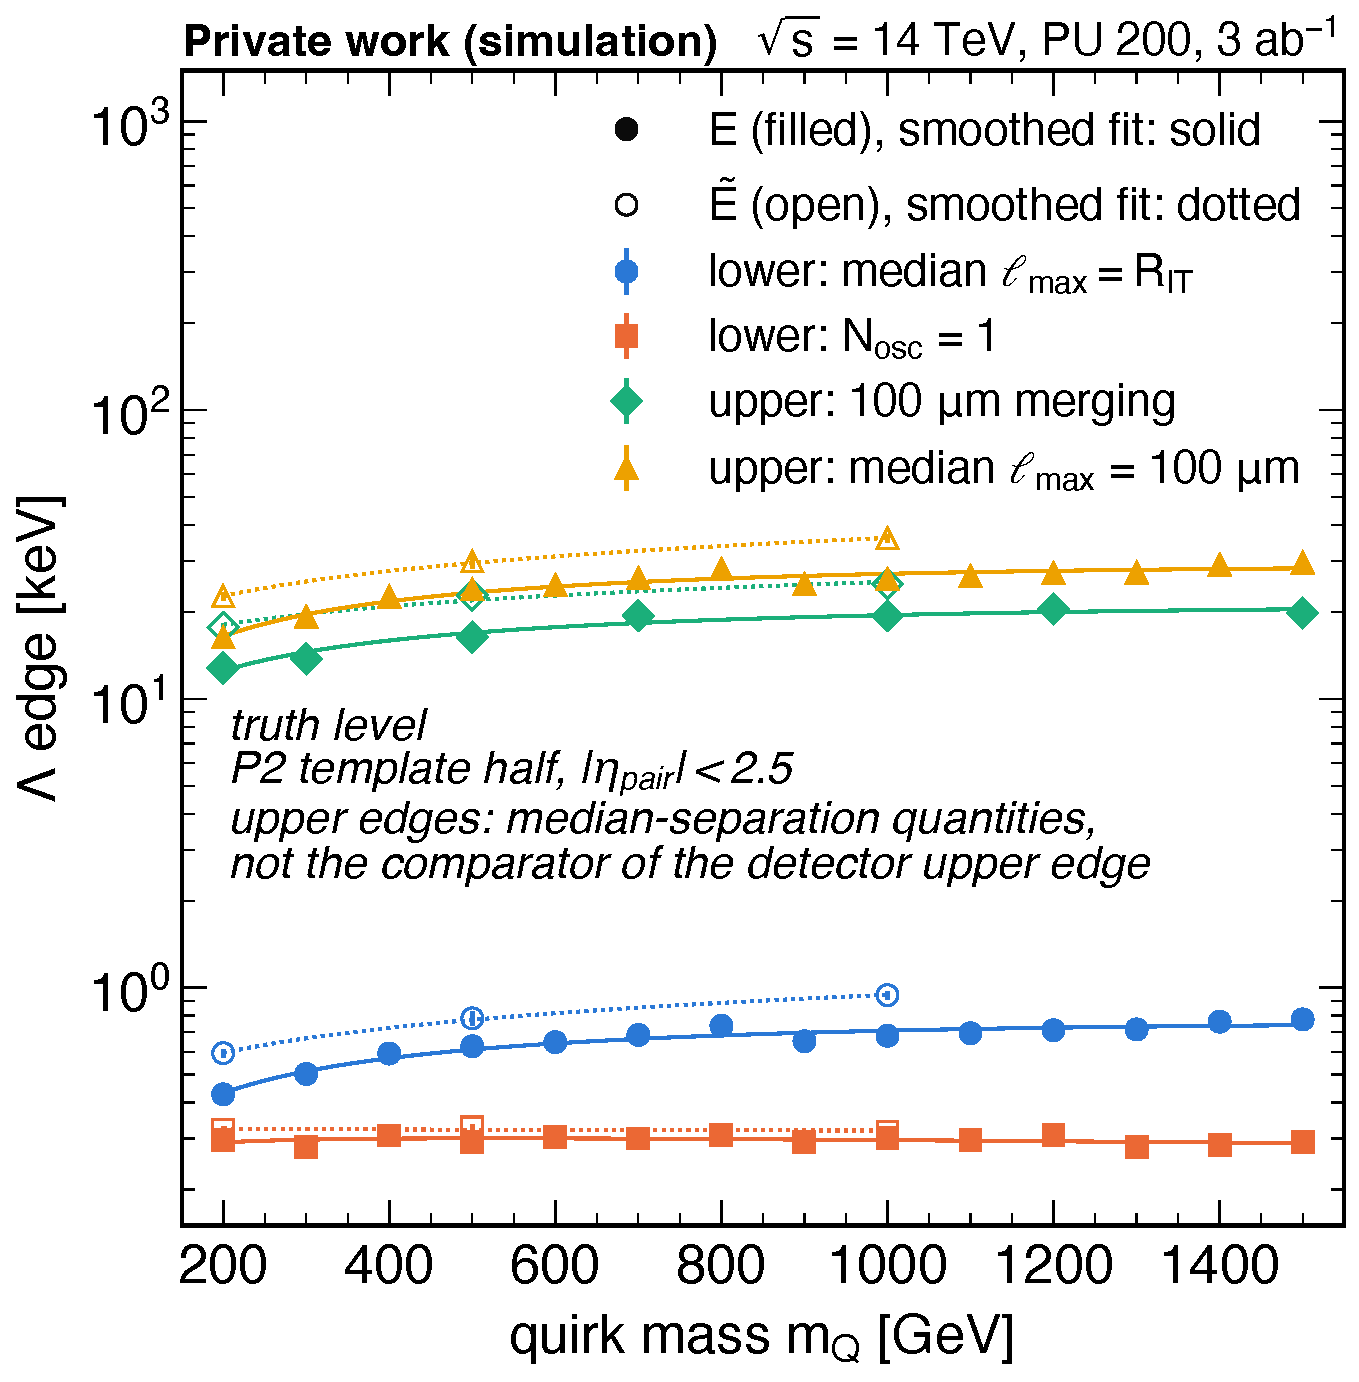
\includegraphics[height=0.37\linewidth]{figures/T4_truth_edges_vs_mass.pdf}
\caption{Truth-level P2 handles (Stage 3, template half, $|\eta_{\rm pair}|<2.5$, field and nominal material; no pile-up,
no resolution). (Left) Median separation $\sepIT$ of the two quirks in the IT against $\Lam$ for five (species, mass)
points (dotted: $\propto\Lam^{-2}$; one panel of the Stage-3 diagnostic figure \rep{sim/stage3/figures/p2_observables.png}):
it follows $\Lam^{-2}$ and so measures $\mQ/\Lam^2$. (Right) $\Lam$ edges against the quirk mass (filled markers and
solid fits: $E$; open markers and dotted fits: $\Etil$): lower edges at median $\lmax=\RIT$ and $\Nosc=1$; upper edges at
50\% of pairs with $\sepIT<100\um$ (hit merging) and at median $\lmax=100\um$. The upper edges are median-separation
quantities, not the comparator of the detector-level upper edge (Section~\ref{sec:mlam:det}); the smoothed lower edge
$\Lam_R(\mQ)$ defines the width admissibility of the fallback (Section~\ref{sec:strategy:fallback}).}
\label{fig:edges}
\end{figure}

\subsection{Detector-level $\Lam$ handles}\label{sec:mlam:det}
At detector level $\Lam$ is constrained only through where the efficiency turns on and off and, without pile-up, through
the measured pair separation. The edges are the half-maximum points of $\Eff$(R04) in $\ln\Lam$, with row-level bootstrap
errors (Figure~\ref{fig:edgesdet}, left).
\begin{itemize}
\item \textbf{Lower edge.} Without pile-up it lies at 0.61/0.65/0.76/0.71/0.85\,keV ($E$ 200/500/1000/1500, $\Etil$ 500),
  equal to the truth edge median $\lmax=\RIT$ within $\approx10\%$ except at $200\GeV$ ($\times1.4$, where wide slow ribbons
  need more than $\lmax<\RIT$). At pile-up 200 it moves up to 1.0--1.2\,keV: wide ribbons lose to pile-up.
\item \textbf{Upper edge.} Without pile-up it lies at 4.7/5.4/5.9/6.1/6.6\,keV. \textbf{The pre-declared truth comparator,
  the 12.8--25\,keV hit-merging edge of Section~\ref{sec:mlam:truth}, is not met} (it is 2.7--3.5 times higher). A comparator
  derived afterwards, the $\Lam$ at which half of the pairs have a merged pair of hits on at least one inner surface
  ($\approx4.5$--$5.5\keV$), agrees within $\approx1\keV$: R04 needs every surface unmerged, and the separation oscillates
  through zero, so some surface merges long before the median separation reaches $100\um$. This agreement is post hoc. At
  pile-up 200 no upper edge exists below $5\keV$, the end of the grid.
\item \textbf{Pair separation.} Without pile-up the measured $\sepIT$ follows the truth within $\approx10\%$ at 1.5--3\,keV
  (e.g.\ $E$ 500 at $2\keV$: 6.9 against 7.0\,mm), saturates at 20--45\,mm below $\approx1\keV$ and sits on a resolution floor
  above $5\keV$ (Figure~\ref{fig:edgesdet}, right). \textbf{At pile-up 200 it is not measurable}: the core-hit median is flat at
  $\approx18$--26\,mm for $\Lam\ge1.5\keV$ while the truth falls from 23 to 0.6\,mm, because pile-up hits define the candidate
  plane. The $\Lam^{-2}$ handle of Section~\ref{sec:mlam:truth} does not survive pile-up with this estimator.
\end{itemize}

\begin{figure}[htbp]
\centering
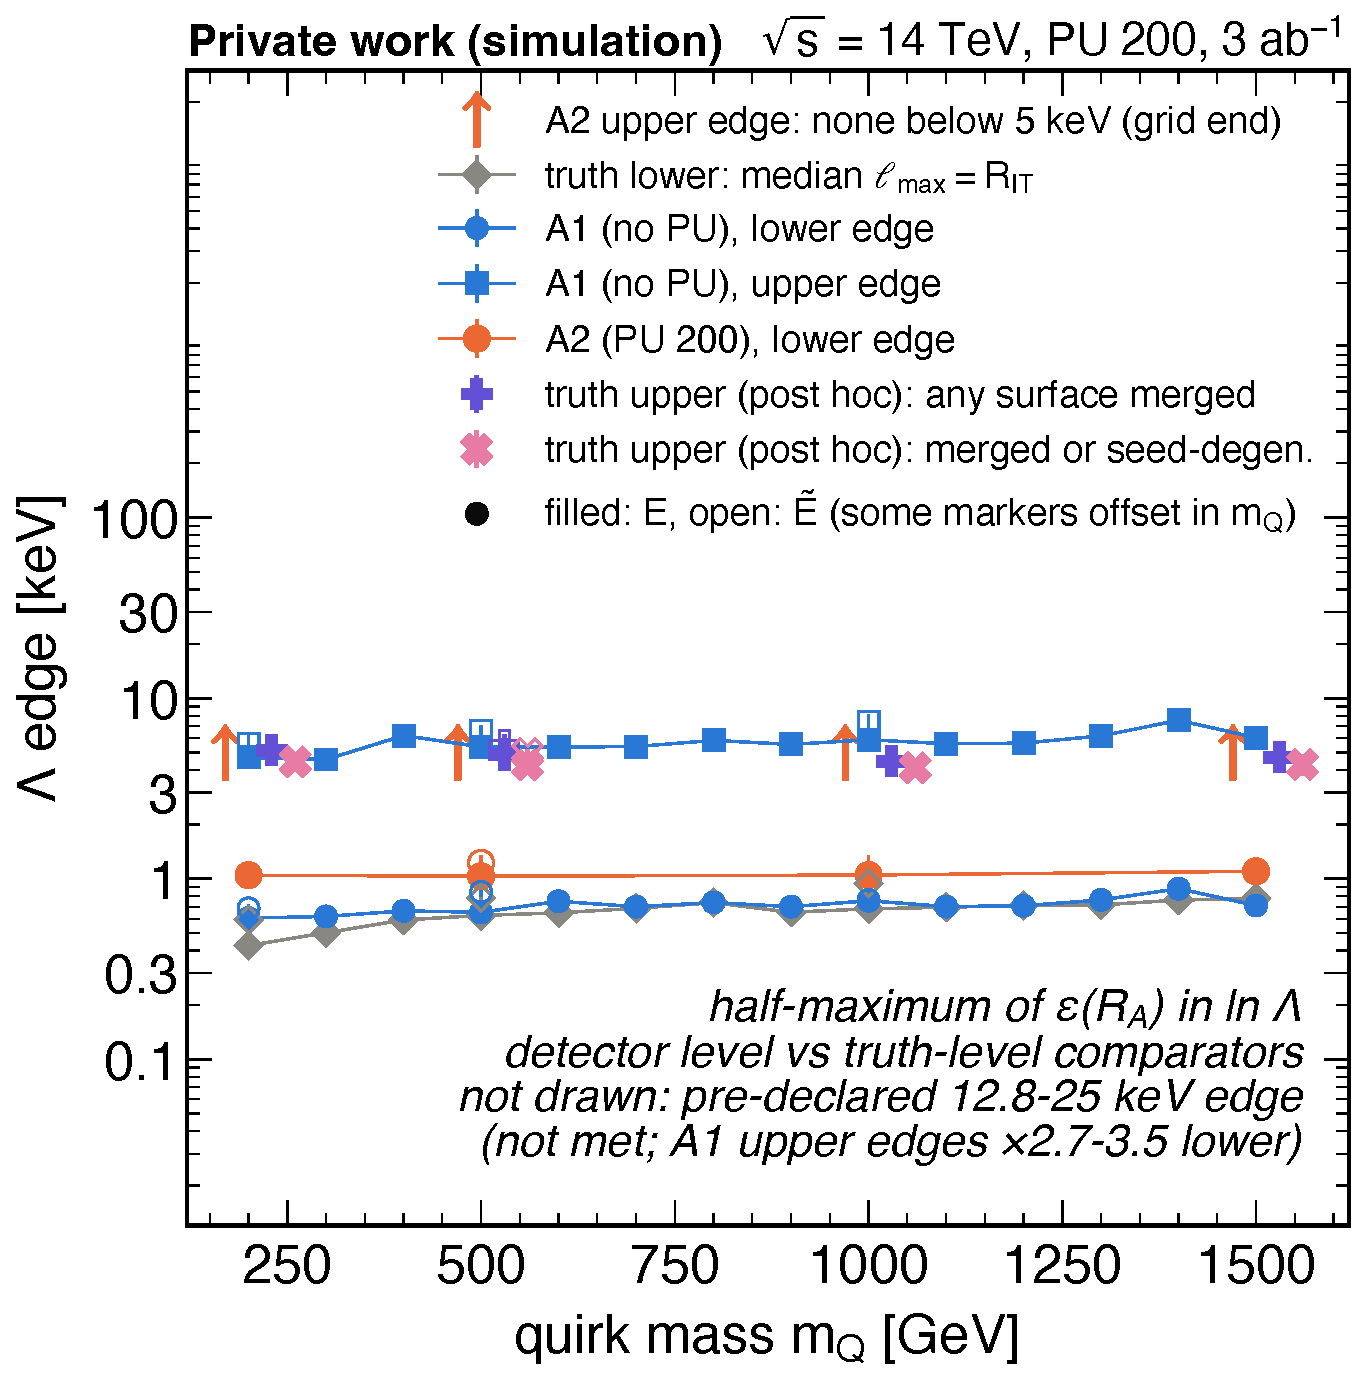
\includegraphics[height=0.37\linewidth]{figures/D9_edges_det_vs_truth.pdf}\hspace{0.02\linewidth}
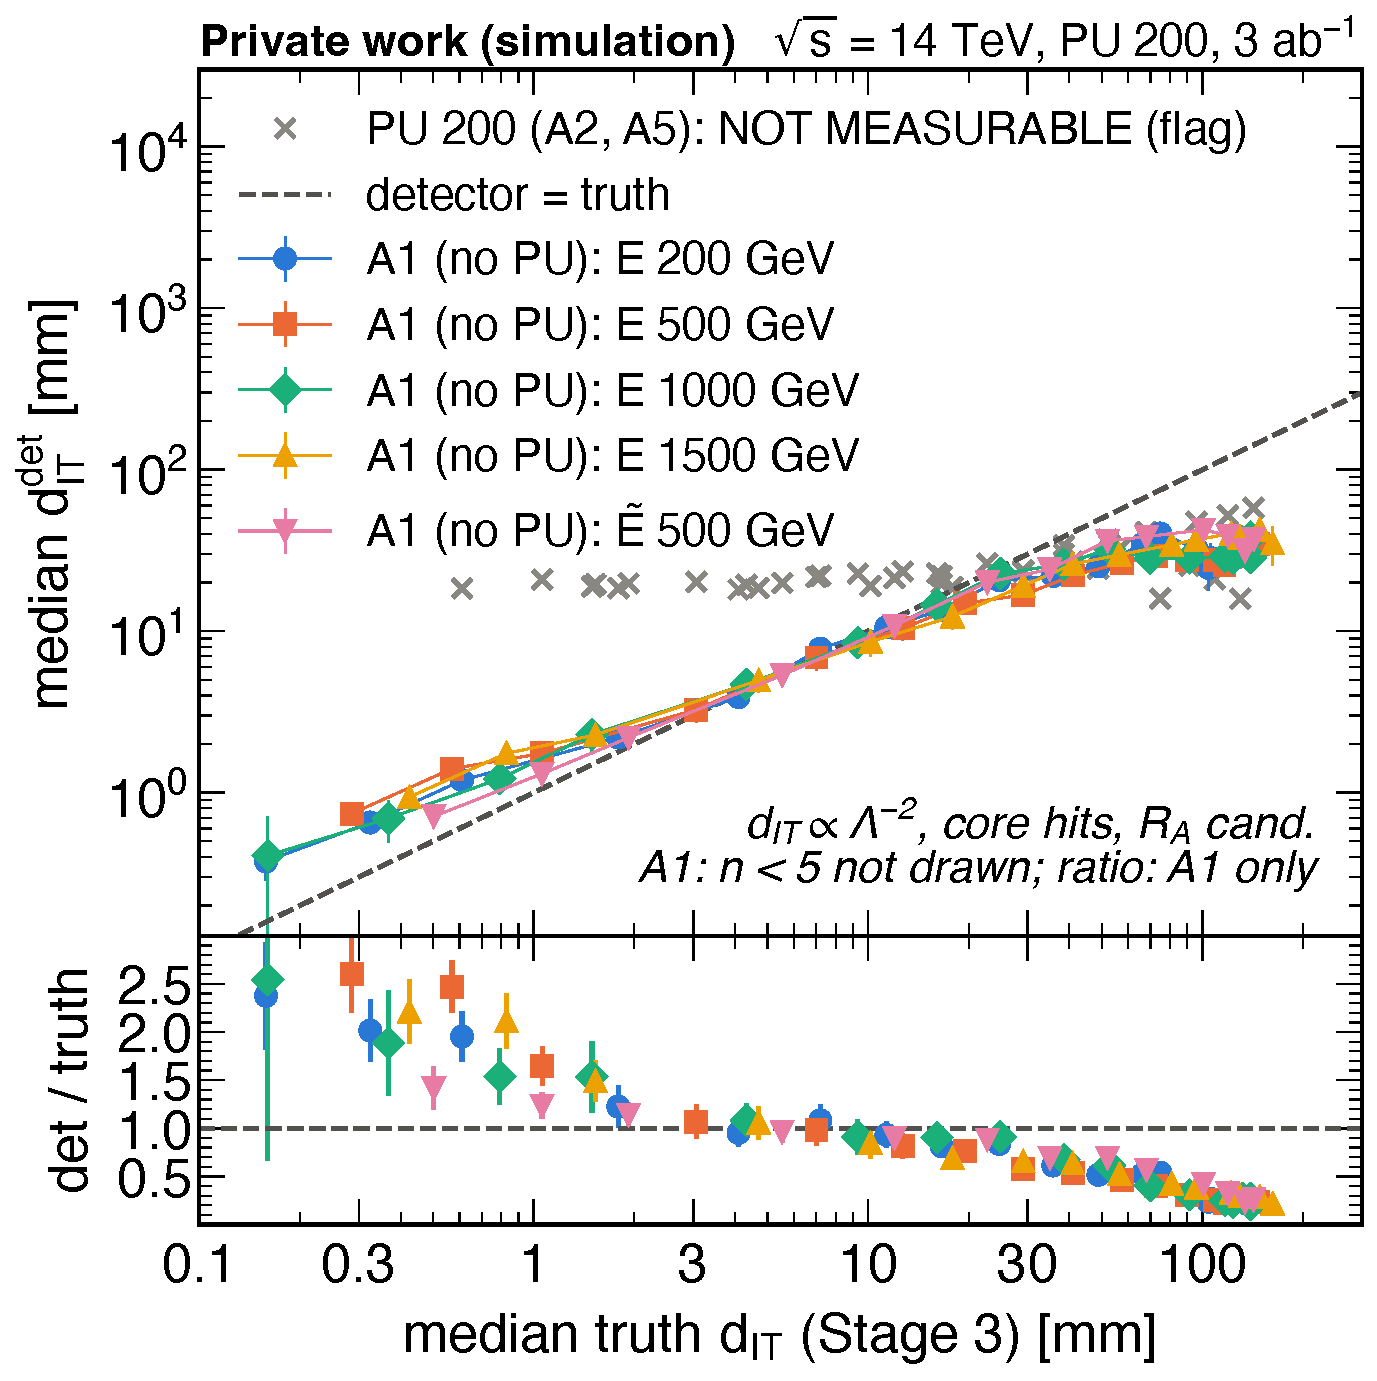
\includegraphics[height=0.37\linewidth]{figures/D10_sepit_calibration.pdf}
\caption{Detector-level $\Lam$ handles. (Left) Half-maximum edges of $\Eff$(R04) in $\ln\Lam$ against $\mQ$: lower and upper
edges without pile-up (A1), lower edges at PU 200 (A2; no upper edge below $5\keV$, arrows), and truth comparators (lower:
median $\lmax=\RIT$; upper, derived post hoc: 50\% of pairs with a merged surface, or merged or seed-degenerate). The
pre-declared 12.8--25\,keV comparator is not drawn and is not met. (Right) Median measured IT pair separation against the
truth: without pile-up (coloured) it tracks the truth at 3--20\,mm; at PU 200 (grey) it is flat and flagged not measurable.}
\label{fig:edgesdet}
\end{figure}

\subsection{Detector-level mass handles}\label{sec:mlam:mass}
The pre-declared mass estimator combines the MET with the pair velocity measured by time of flight to the barrel timing
layer, $M_{\rm est}=\mathrm{MET}\cosh\eta_{\rm axis}/(\beta\gamma)_{\rm ToF}$ (user decision). Since $\mathrm{MET}\cosh\eta$
approximates the pair momentum, $M_{\rm est}$ estimates the \textbf{pair mass $M_{Q\bar Q}\ge2\mQ$, not $\mQ$}.
Figure~\ref{fig:mest} shows its distribution at R04 for two masses.
\begin{itemize}
\item \textbf{Without pile-up} no event falls below $1.5\mQ$ (0 of 9551; minimum $1.69\mQ$), and the pooled median is
  $2.46\mQ$, just above the threshold $2\mQ$.
\item \textbf{At pile-up 200} the pooled median is $2.26\mQ$ (850 events with a defined $M_{\rm est}$), but 29\% of the
  events fall below $1.5\mQ$ and 19\% below $0.5\mQ$: a low cluster from in-time pile-up timing hits, which make
  $\beta_{\rm ToF}\to1$. $M_{\rm est}$ is undefined for 6--41\% of the candidates. The per-mass medians keep the mass
  ordering (483/1113/2070/3137\,GeV for $E$ 200/500/1000/1500), but the 16\% quantiles are 155--332\,GeV for every mass.
\item \textbf{$\beta_{\rm ToF}$ and $dE/dx$.} The median $\beta_{\rm ToF}$ rises from 0.23--0.53 without pile-up to 0.39--0.68
  with it; the truncated-mean $dE/dx$ is diluted from 1.8--7.1 to 1.5--2.7 MIP and keeps only a weak mass ordering.
\item \textbf{$\wcore$ as the $\lmax$ observable.} Without pile-up its median falls monotonically with $\Lam$ above
  $\approx0.85\keV$ ($E$ 500: 13.1/5.5/2.4/1.3\,mm at 1/2/3/5\,keV); at pile-up 200 it flattens to $\approx10$--12\,mm at
  $\ge3\keV$, because pile-up hits enter the core.
\end{itemize}
\textbf{P2 verdict on $\mQ$ and $\Lam$.} At pile-up 200 this set-up measures neither $\mQ$ nor $\Lam$: it provides an
ordering of the masses through the pair-mass proxy, and brackets $\Lam$ by the efficiency window. No mass fit or template
was run. A pile-up-robust separation estimator and a timing selection that rejects in-time pile-up hits would be needed to
recover the truth-level handles.

\begin{figure}[htbp]
\centering
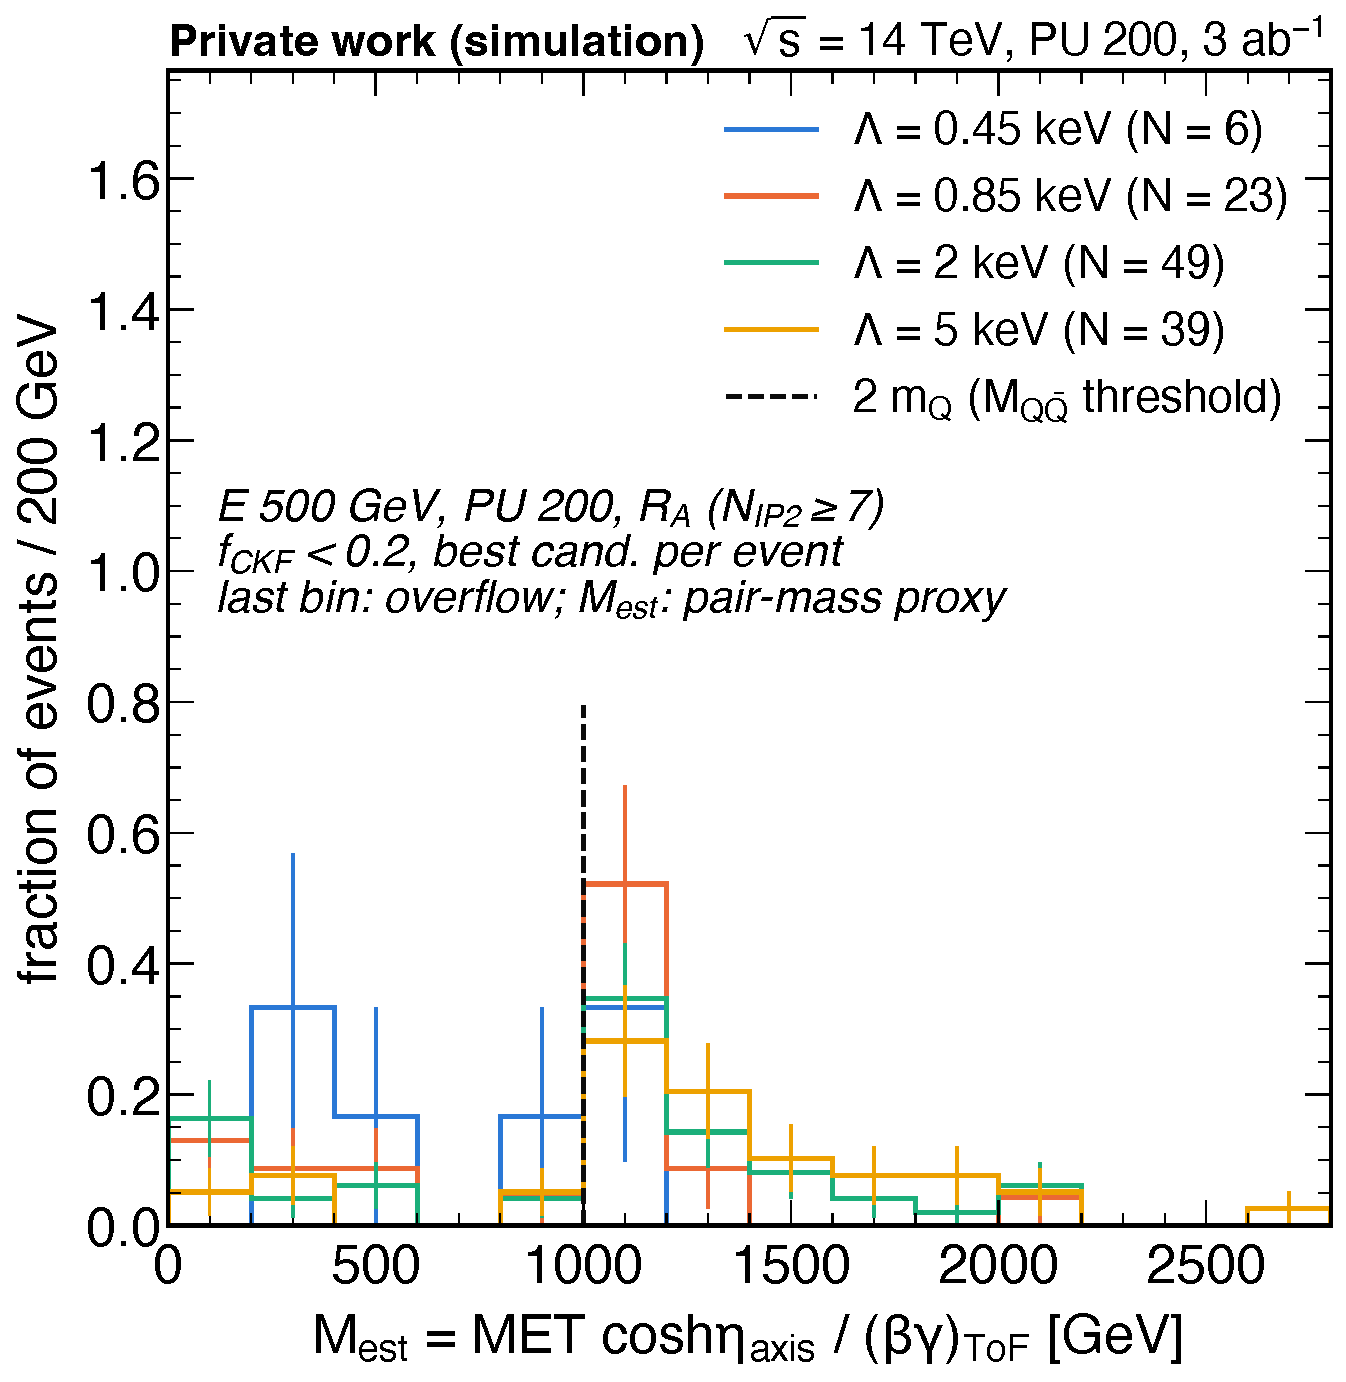
\includegraphics[height=0.38\linewidth]{figures/D8_mest_RA_F500.pdf}\hspace{0.02\linewidth}
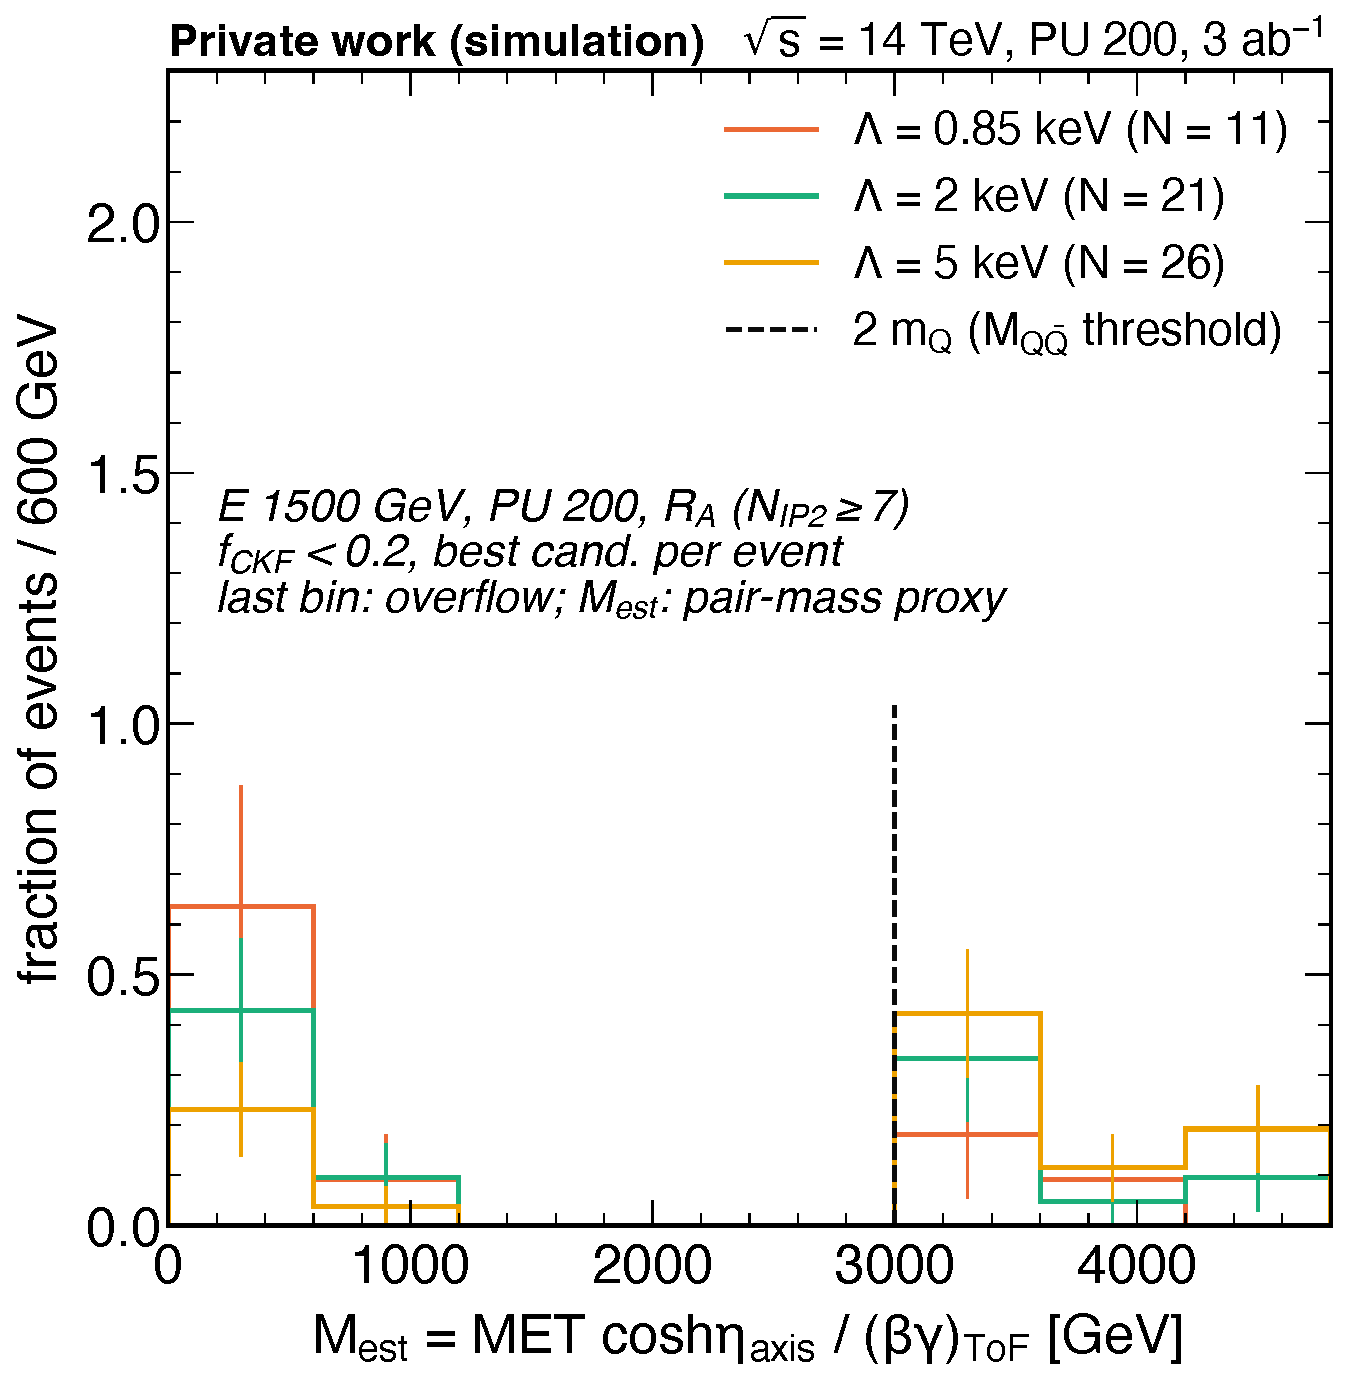
\includegraphics[height=0.38\linewidth]{figures/D8_mest_RA_F1500.pdf}
\caption{Distribution of the pair-mass proxy $M_{\rm est}=\mathrm{MET}\cosh\eta_{\rm axis}/(\beta\gamma)_{\rm ToF}$ at
detector level (PU 200, selection R04, best candidate per event, $f_{\rm CKF}<0.2$) for $E$ at 500 (left) and $1500\GeV$
(right), for several $\Lam$; the dashed line is $2\mQ$. The upper cluster starts near the pair-mass threshold $2\mQ$; the low
cluster at 0.1--0.4\,$\mQ$ comes from in-time pile-up timing hits. Nothing is expected near $\mQ$ itself. Per curve only
6--49 events enter, so the shapes are statistically weak.}
\label{fig:mest}
\end{figure}
